\section{Gebruikersinterface}

De gebruikersinterface maakt het inzichtelijk op een kaart waar de door de
SmartMarkers gemeten punten zich bevinden. Daarnaast is het mogelijk om op
deze kaart percelen aan te maken, om de meetpunten ook daadwerkelijk te
gebruiken.

\subsection*{Eerste weergave}
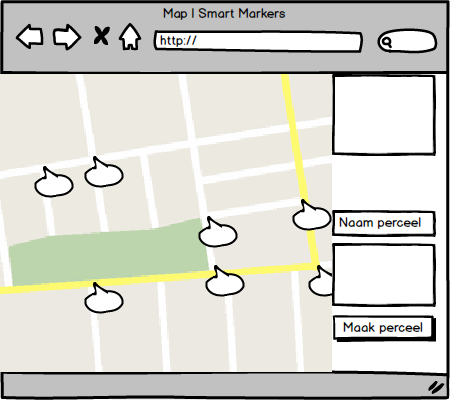
\includegraphics{functional/map_1.png}
Wanneer de wegpagina bezocht wordt, toont deze een kaart met de daarop reeds
ontvangen meetpunten uit de database.

\subsection*{Meetpunt selecteren}
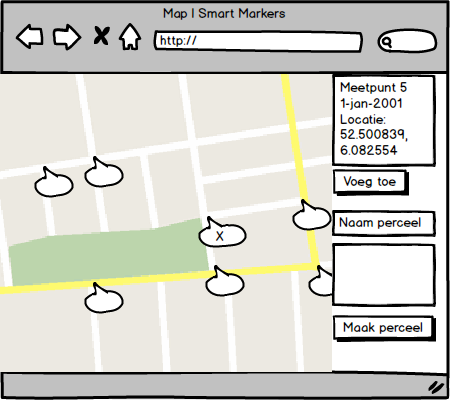
\includegraphics{functional/map_2.png}
Wanneer één van de meetpunten geselecteerd is, wordt in de informatiebox
rechtsboven de beschikbare informatie als naam, locatie en tijdstip van meten
getoond.
Daarnaast komt er een 'Voeg toe' button in beeld, welke het mogelijk
maakt om een X aantal meetpunten aan een lijst met meetpunten voor een nieuw
te maken perceel toe te voegen.

\subsection*{Perceel aanmaken}
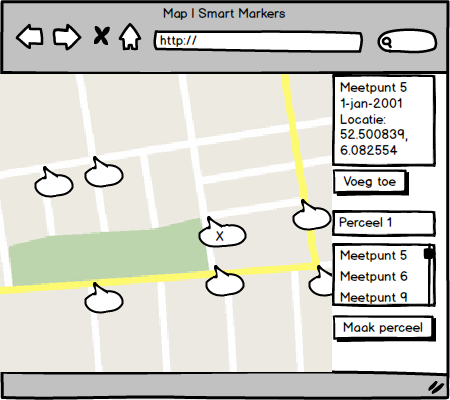
\includegraphics{functional/map_3.png}
De tekstbox met 'Naam perceel' kan gebruikt worden om een naam voor het perceel
in te geven. Daarnaast is een lijst gemaakt van toegevoegde meetpunten. Door op
de 'Maak perceel' button te klikken wordt de huidige selectie, met naam, als een
nieuw perceel op de kaart weergegeven

\subsection*{Perceel aangemaakt}
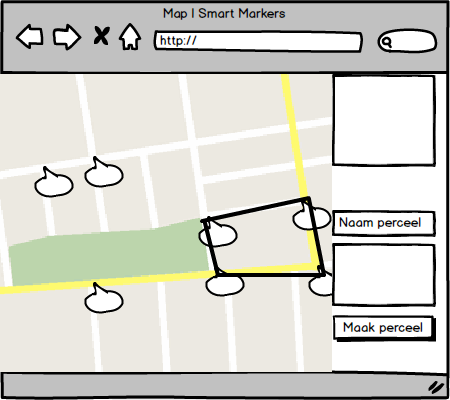
\includegraphics{functional/map_4.png}
Na het op 'Maak perceel' klikken, wordt scherm gelijk aan de eerste weergave
getoond, met het verschil dat het zojuist gemaakte perceel nu zichtbaar gemarkeerd
op de kaart getoond wordt.

\subsection*{Perceel selecteren}
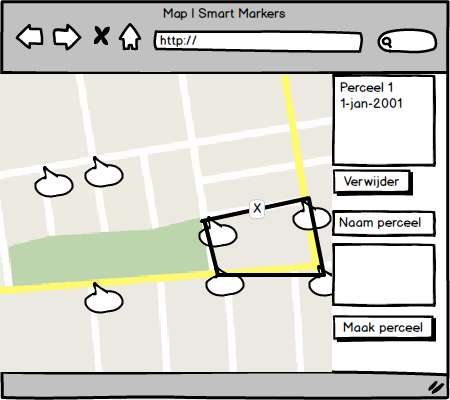
\includegraphics{functional/map_5.png}
Wanneer één van de gemaakte percelen geselecteerd is, wordt in de informatiebox
rechtsboven de naam en het tijdstip van creëren van het perceel getoond.
Daarnaast komt er een 'Verwijder' button in beeld, welke het mogelijk maakt het
geselecteerde perceel te verwijderen. Door hier op te klikken wordt dit perceel
uit de database verwijderd.
